\section{Evidencia de reversión a la media y calibración del Log-OU}
\label{sec:results_logou}

La primera etapa evalúa si la dinámica observada del precio H100 es compatible con el
Log-OU utilizado posteriormente para construir el entorno sintético de valoración. El
objetivo no es identificar un modelo ``verdadero'' del mercado de cómputo, sino comprobar
si una especificación parsimoniosa con reversión a la media resulta defendible con la
evidencia disponible y cuantificar la incertidumbre de calibración.

Sobre las 92 observaciones diarias de Ornn, la estimación
$Y_{t+1}=a+\phi Y_t+\varepsilon_{t+1}$, con $Y_t=\log P_t$, proporciona
$\widehat a=0{,}08498$, $\widehat\phi=0{,}91440$ y $R^2=0{,}8145$. El intervalo
convencional al 95\% de $\phi$, $[0{,}8225,1{,}0063]$, contiene la unidad.
Asimismo, el ADF no rechaza raíz unitaria ($p=0{,}356$), mientras que el KPSS
tampoco rechaza estacionariedad ($p\geq0.10$). En consecuencia, el valor puntual es
compatible con reversión a la media, pero la corta muestra no permite establecer de forma
concluyente la estacionariedad del nivel logarítmico.
\begin{align}
    \widehat\phi &= 0.91440, \label{eq:result_phi}\\
    IC_{95\%}(\phi) &= [0.8225,1.0063]. \label{eq:phi_ci}
\end{align}

La transformación exacta de AR(1) a Log-OU conduce a los parámetros de la
Tabla~\ref{tab:logou_calibration_results}. La velocidad de reversión estimada implica una
vida media de 7{,}75 días, lo que constituye una reversión económicamente rápida dentro de
la especificación.
\begin{align}
    \widehat\kappa_P &= 32.6645, \label{eq:result_kappa}\\
    \widehat\vartheta_P &= 0{,}99269,\qquad
    \exp(\widehat\vartheta_P)=2.6985, \label{eq:result_long_run_level}\\
    \widehat\sigma_P &= 0.6247, \label{eq:result_sigma}\\
    t_{1/2} &= 7.75\ \text{días}. \label{eq:result_half_life}
\end{align}

\begin{table}[htbp]
    \centering
    \caption{Calibración física del modelo Log-OU sobre Ornn H100.}
    \label{tab:logou_calibration_results}
    \begin{tabular}{lr}
        \toprule
        Magnitud & Estimación \\
        \midrule
        Observaciones & 92 \\
        Intercepto AR(1), $\widehat a$ & 0{,}08498 \\
        Persistencia, $\widehat\phi$ & 0{,}91440 \\
        $IC_{95\%}$ de $\phi$ & $[0{,}8225,\,1{,}0063]$ \\
        $R^2$ AR(1) & 0{,}8145 \\
        $\widehat\kappa_P$ anual & 32{,}6645 \\
        $\widehat\vartheta_P$ & 0{,}99269 \\
        $\exp(\widehat\vartheta_P)$ & 2{,}6985 \\
        $\widehat\sigma_P$ anual & 0{,}6247 \\
        Vida media & 7{,}75 días \\
        \bottomrule
    \end{tabular}
\end{table}

Como contraste predictivo, una evaluación \textit{expanding one-step} del log-precio
produce un RMSE de 0{,}03161 para AR(1), frente a 0{,}03209 para un random walk, y un
MAE de 0{,}02384 frente a 0.02466. Las mejoras, 1{,}50\% y 3{,}34\%,
respectivamente, son positivas pero moderadas. Los contrastes HAC de diferencia de pérdidas dan $p=0{,}145$ para pérdida cuadrática
y $p=0{,}0627$ para absoluta; no establecen superioridad al 5\%.
Esta evidencia justifica utilizar Log-OU
como modelo principal parsimonioso, no descartar dinámicas alternativas.

La incertidumbre paramétrica se cuantifica mediante 20\,000 réplicas bootstrap
residuales, de las que se conservan 19\,994 estacionarias y se descartan seis.
La Tabla~\ref{tab:bootstrap_logou_results} muestra que la dispersión es
especialmente elevada en $\kappa$. El rango P10--P90 se utiliza para informar, y no
identificar, el dominio sintético de valoración.

\begin{table}[htbp]
    \centering
    \caption{Sensibilidad bootstrap de los parámetros Log-OU.}
    \label{tab:bootstrap_logou_results}
    \begin{tabular}{lrrr}
        \toprule
        Rango central & $\kappa$ & $\sigma$ & Vida media (días) \\
        \midrule
        P10--P90
        & $[25{,}055,\,87{,}047]$
        & $[0{,}5508,\,0{,}7119]$
        & $[2{,}91,\,10{,}10]$ \\
        P5--P95
        & $[20{,}523,\,102{,}382]$
        & $[0{,}5279,\,0{,}7357]$
        & $[2{,}47,\,12{,}33]$ \\
        P2.5--P97.5
        & $[17{,}240,\,117{,}480]$
        & $[0{,}5100,\,0{,}7542]$
        & $[2{,}15,\,14{,}67]$ \\
        \bottomrule
    \end{tabular}
\end{table}

De acuerdo con el protocolo del Capítulo~\ref{chap:metodologia}, los rangos de diseño
se fijan como
\begin{equation}
    \kappa_Q\in[25,87],
    \qquad
    \sigma_Q\in[0{,}55,0{,}71],
    \label{eq:result_frozen_dynamic_domain}
\end{equation}
mientras que el nivel de largo plazo se normaliza alrededor de
$K_{\mathrm{ref}}=2{,}6985$ y los extremos observados de Ornn determinan
\begin{equation}
    \theta_Q\in[-0{,}1641,0{,}1610].
    \label{eq:result_theta_domain}
\end{equation}
Estos intervalos son \emph{bandas de diseño} para explorar riesgo de modelo; no son
intervalos de confianza de parámetros neutrales al riesgo. La evidencia histórica bajo
$\mathbb P$ informa la elección del dominio, pero no identifica por sí sola la dinámica
bajo la medida de valoración modelizada $\mathbb Q$.

\section{Resultados de valoración: MLP frente a DML}
\label{sec:resultados_pricing}

La comparación principal utiliza pares MLP--DML entrenados con las mismas muestras,
semillas e hiperparámetros congelados; la diferencia sistemática es la supervisión
diferencial de DML. La Tabla~\ref{tab:pricing_test_results} recoge el error del precio
normalizado en test para los cuatro tamaños de entrenamiento.

\begin{table}[htbp]
\centering
\scriptsize
\setlength{\tabcolsep}{4pt}
\caption{Error de valoración en el conjunto de test}
\label{tab:pricing_test_results}
\begin{tabular}{lcccc}
\toprule
\textbf{$N_{\mathrm{train}}$}
& \textbf{RMSE MLP}
& \textbf{RMSE DML}
& \textbf{MAE MLP}
& \textbf{MAE DML} \\
\midrule
$1\,024$
& $0{,}009217 \pm 0{,}000034$
& $0{,}009232 \pm 0{,}000045$
& $0{,}005961 \pm 0{,}000071$
& $0{,}005911 \pm 0{,}000114$ \\
$4\,096$
& $0{,}008747 \pm 0{,}000009$
& $0{,}008767 \pm 0{,}000039$
& $0{,}005330 \pm 0{,}000041$
& $0{,}005326 \pm 0{,}000079$ \\
$16\,384$
& $0{,}008438 \pm 0{,}000013$
& $0{,}007610 \pm 0{,}001995$
& $0{,}005002 \pm 0{,}000022$
& $0{,}004316 \pm 0{,}001636$ \\
$65\,536$
& $0{,}001624 \pm 0{,}000043$
& $0{,}001516 \pm 0{,}000130$
& $0{,}000123 \pm 0{,}000025$
& $0{,}000136 \pm 0{,}000046$ \\
\bottomrule
\end{tabular}
\par\smallskip{\scriptsize Nota: media $\pm$ desviación muestral entre cinco semillas sobre los mismos estados.}
\end{table}

Con 1\,024 y 4\,096 estados las diferencias son reducidas. Con 16\,384,
DML presenta menor error medio, pero elevada dispersión entre semillas y sólo obtiene menor
RMSE en uno de los cinco pares, por lo que no se interpreta como una mejora sistemática.
La configuración final de 65\,536 estados es más estable: DML reduce el RMSE de
0{,}001624 a 0{,}001516 (aproximadamente 6{,}7\%) y gana cuatro de cinco
comparaciones emparejadas. En cambio, el MLP obtiene menor MAE:
$1{,}226\times10^{-4}$ frente a $1{,}356\times10^{-4}$, de modo que el MAE de DML es aproximadamente un 10{,}6\% mayor que el de MLP;
MLP gana tres de cinco pares. Por tanto,
\begin{equation}
    \operatorname{RMSE}_{DML}<\operatorname{RMSE}_{MLP},
    \qquad
    \operatorname{MAE}_{DML}>\operatorname{MAE}_{MLP}.
    \label{eq:pricing_mixed_result}
\end{equation}
La diferencia entre MAE y RMSE anticipa una distribución del error distinta, analizada en
la Sección~\ref{sec:extreme_errors}.

El conjunto de referencia, construido con dieciséis aleatorizaciones RQMC por estado,
favorece más claramente a DML en la configuración final: el RMSE pasa de 0{,}001163
(MLP) a 0{,}000801 (DML), una media de reducciones emparejadas de aproximadamente el 30{,}4\% y
cinco de cinco pares favorables. El MAE es 0{,}000128 frente a 0{,}000116, aunque DML
sólo gana tres de cinco pares. En conjunto, DML mantiene una precisión de pricing
comparable y mejora algunas métricas, especialmente el RMSE final y de referencia, pero
\textbf{no domina uniformemente la valoración}.

\section{Precisión de Delta y eficiencia muestral}
\label{sec:delta_sample_efficiency}

La diferencia entre modelos es mucho más clara en Delta. La
Tabla~\ref{tab:delta_test_results} muestra que DML obtiene menor MAE y RMSE que MLP
en las cinco semillas para los cuatro tamaños de entrenamiento.

\begin{table}[htbp]
\centering
\small
\caption{Error de Delta en el conjunto de test}
\label{tab:delta_test_results}
\resizebox{\textwidth}{!}{%
\begin{tabular}{lccccc}
\toprule
\textbf{$N_{\mathrm{train}}$}
& \textbf{MAE MLP}
& \textbf{MAE DML}
& \textbf{RMSE MLP}
& \textbf{RMSE DML}
& \textbf{DML mejor} \\
\midrule
$1\,024$
& $0{,}020884 \pm 0{,}001163$
& $0{,}010468 \pm 0{,}002188$
& $0{,}029881 \pm 0{,}001880$
& $0{,}014870 \pm 0{,}002114$
& $5/5$ \\
$4\,096$
& $0{,}018047 \pm 0{,}001601$
& $0{,}006254 \pm 0{,}000112$
& $0{,}026927 \pm 0{,}003220$
& $0{,}011204 \pm 0{,}000132$
& $5/5$ \\
$16\,384$
& $0{,}013890 \pm 0{,}000487$
& $0{,}005232 \pm 0{,}001798$
& $0{,}020542 \pm 0{,}000552$
& $0{,}009674 \pm 0{,}002136$
& $5/5$ \\
$65\,536$
& $0{,}001234 \pm 0{,}000264$
& $0{,}000216 \pm 0{,}000085$
& $0{,}008528 \pm 0{,}001257$
& $0{,}001817 \pm 0{,}000245$
& $5/5$ \\
\bottomrule
\end{tabular}
}
\par\smallskip{\scriptsize Nota: media $\pm$ desviación muestral entre cinco semillas sobre los mismos estados.}
\end{table}

\begin{figure}[htbp]
    \centering
    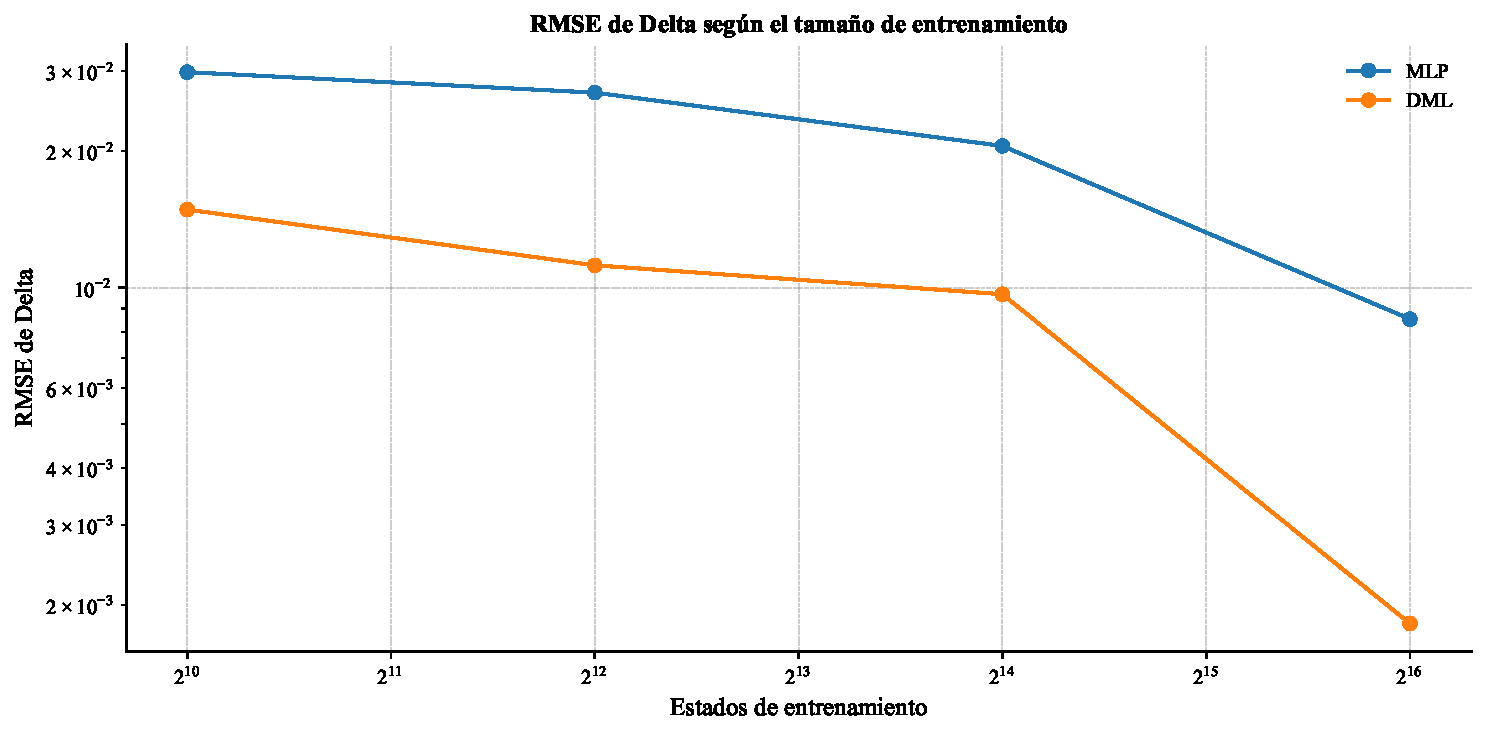
\includegraphics[width=0.88\textwidth]{../figures/ml/03_delta_rmse_learning_curve.pdf}
    \caption{RMSE de Delta en test según el tamaño del conjunto de entrenamiento.}
    \label{fig:delta_rmse_learning_curve}
\end{figure}

En la configuración de 65\,536 estados, DML reduce el MAE de 0{,}001234 a
0{,}000216 y el RMSE de 0{,}008528 a 0.001817. Las reducciones emparejadas
medias son, respectivamente, 82{,}0\% y 78{,}5\%. El $R^2$ de Delta pasa de
0{,}7603 para MLP a 0{,}9891 para DML. La mejora se reproduce en el conjunto de
referencia: MAE de 0{,}001404 frente a 0{,}000198 y RMSE de 0{,}009372 frente a
0{,}001158, con cinco de cinco pares favorables.

Las curvas de aprendizaje aportan además evidencia de mayor eficiencia muestral. DML con
1\,024 estados alcanza MAE 0{,}010468 y RMSE 0{,}014870, ambos inferiores a los
0{,}013890 y 0{,}020542 del MLP entrenado con 16\,384 estados. Este resultado demuestra
que, \emph{dentro de la malla experimental}, DML puede alcanzar mayor precisión de Delta
con sustancialmente menos estados; no implica una tasa universal de eficiencia de 16 veces.
La misma ordenación se reproduce en referencia.

Esta eficiencia muestral tampoco equivale a menor coste de entrenamiento. En la
configuración final, los tiempos medios son aproximadamente 2\,494 s para MLP y
3\,363 s para DML, de modo que la supervisión diferencial incrementa el tiempo cerca de
un 35\%. La ventaja consiste en extraer más información útil de cada estado de
entrenamiento, especialmente sobre la sensibilidad de la función de valoración.

\section{Errores extremos de precio y Delta}
\label{sec:extreme_errors}

Los percentiles superiores permiten determinar si las diferencias de error proceden del
comportamiento general o de una fracción reducida de estados. La
Tabla~\ref{tab:pricing_tail_errors} resume P95, P99 y máximo para la configuración final.

\begin{table}[htbp]
\centering
\small
\caption{Colas del error absoluto de precio y Delta en test,
$N_{\mathrm{train}}=65\,536$}
\label{tab:pricing_tail_errors}
\label{tab:delta_tail_errors}
\begin{tabular}{llccc}
\toprule
\textbf{Magnitud} & \textbf{Modelo} & \textbf{P95} & \textbf{P99} & \textbf{Máximo} \\
\midrule
Precio & MLP & $2{,}367\times10^{-4}$ & $6{,}176\times10^{-4}$ & $8{,}389\times10^{-2}$ \\
Precio & DML & $2{,}723\times10^{-4}$ & $5{,}031\times10^{-4}$ & $7{,}677\times10^{-2}$ \\
Delta & MLP & $3{,}262\times10^{-3}$ & $9{,}424\times10^{-3}$ & $0{,}5115$ \\
Delta & DML & $4{,}880\times10^{-4}$ & $1{,}229\times10^{-3}$ & $0{,}0790$ \\
\bottomrule
\end{tabular}
\par\smallskip{\scriptsize Nota: medias de los P95, P99 y máximos de cada ejecución; no son estadísticos globales ni del ensemble.}
\end{table}

En precio, MLP obtiene menor P95, mientras que DML reduce P99 aproximadamente
18{,}5\% y el máximo de 0{,}08389 a 0.07677. Esto es coherente con el menor MAE
del MLP y el menor RMSE de DML: el modelo diferencial no mejora toda la distribución,
pero contiene mejor parte de la cola extrema. El patrón cualitativo se mantiene en el conjunto
de referencia, donde DML también presenta menor P99 y máximo.

En Delta la ventaja es mucho más intensa: DML reduce P95 aproximadamente 85\%, P99
87\% y el máximo 84{,}6\%. En referencia se obtiene una conclusión similar, con máximos
de 0{,}2486 para MLP y 0{,}0337 para DML. Por tanto, la supervisión diferencial mejora no
sólo el error medio de Delta, sino también las regiones más adversas del dominio evaluado.
Los estadísticos de cola no identifican, sin embargo, qué características de los estados
originan esos episodios; esta cuestión motiva el diagnóstico contractual siguiente.

Un diagnóstico posterior de las predicciones finales identifica violaciones de
positividad y monotonicidad: la salida lineal no impone $V\geq0$ ni $\Delta\geq0$.
Sobre 8192 estados de test y cinco semillas (40\,960 predicciones por modelo),
los precios negativos representan el $14{,}73\%$ en MLP y el $13{,}05\%$ en DML;
los mínimos son $-0{,}004049$ y $-0{,}000885$. Las Deltas negativas representan
el $20{,}06\%$ y el $14{,}17\%$, con mínimos $-0{,}241302$ y $-0{,}013681$.
La frecuencia incluye valores próximos a cero; el material reproducible conserva
también conteos por debajo de $-10^{-6}$. No se recortan las predicciones ni se
modifican las métricas principales. La mejora de DML no garantiza restricciones
financieras globales.

\section{Efecto de las fronteras de fixing}
\label{sec:fixing_boundaries}

La opción contiene 12 fixings mensuales. El vector de entrada incorpora el tiempo a
vencimiento, pero no codifica explícitamente ni la distancia a la frontera de fixing más
próxima ni el número de fixings pendientes. Estas variables se conservaron como metadatos,
lo que permite realizar un diagnóstico \textit{post-hoc} sobre los modelos ya congelados,
sin utilizar el test para rediseñar o reentrenar.

Definiendo $d_{\mathrm{fix}}$ como la distancia, en días, a la frontera mensual más próxima,
la mediana del diagnóstico de test es 7{,}54 días; entre los 50 mayores errores de Delta de
DML cae a 0{,}49 días. La Tabla~\ref{tab:fixing_top50} muestra una concentración muy
superior a la frecuencia de estas regiones en la muestra.

\begin{table}[htbp]
\centering
\small
\caption{Concentración de los 50 mayores errores de Delta de DML alrededor
de fronteras de fixing}
\label{tab:fixing_top50}
\begin{tabular}{lccc}
\toprule
\textbf{Distancia}
& \textbf{Muestra total}
& \textbf{Top 50 DML}
& \textbf{Sobrerrepresentación} \\
\midrule
$\leq 0{,}5$ días & $3{,}30\%$ & $52\%$ & $15{,}8\times$ \\
$\leq 1$ día & $6{,}65\%$ & $64\%$ & $9{,}6\times$ \\
$\leq 2$ días & $13{,}27\%$ & $88\%$ & $6{,}6\times$ \\
$\leq 3$ días & $19{,}91\%$ & $92\%$ & $4{,}6\times$ \\
\bottomrule
\end{tabular}
\end{table}

El patrón aparece también al agrupar el error medio por distancia. A menos de medio día
de una frontera, el MAE de Delta es 0{,}005153 para MLP y 0{,}001742 para DML; a más
de tres días cae a 0{,}000832 y 0{,}000128, respectivamente.

\begin{table}[htbp]
\centering
\small
\caption{Error absoluto medio de Delta según distancia a una frontera de fixing}
\label{tab:delta_fixing_distance}
\begin{tabular}{lccc}
\toprule
\textbf{Distancia}
& \textbf{$n$}
& \textbf{MLP}
& \textbf{DML} \\
\midrule
$\leq 0{,}5$ días & $270$ & $0{,}005153$ & $0{,}001742$ \\
$(0{,}5,1]$ días & $275$ & $0{,}003835$ & $0{,}000506$ \\
$(1,3]$ días & $1\,086$ & $0{,}002034$ & $0{,}000295$ \\
$>3$ días & $6\,561$ & $0{,}000832$ & $0{,}000128$ \\
\bottomrule
\end{tabular}
\end{table}

\begin{figure}[htbp]
    \centering
    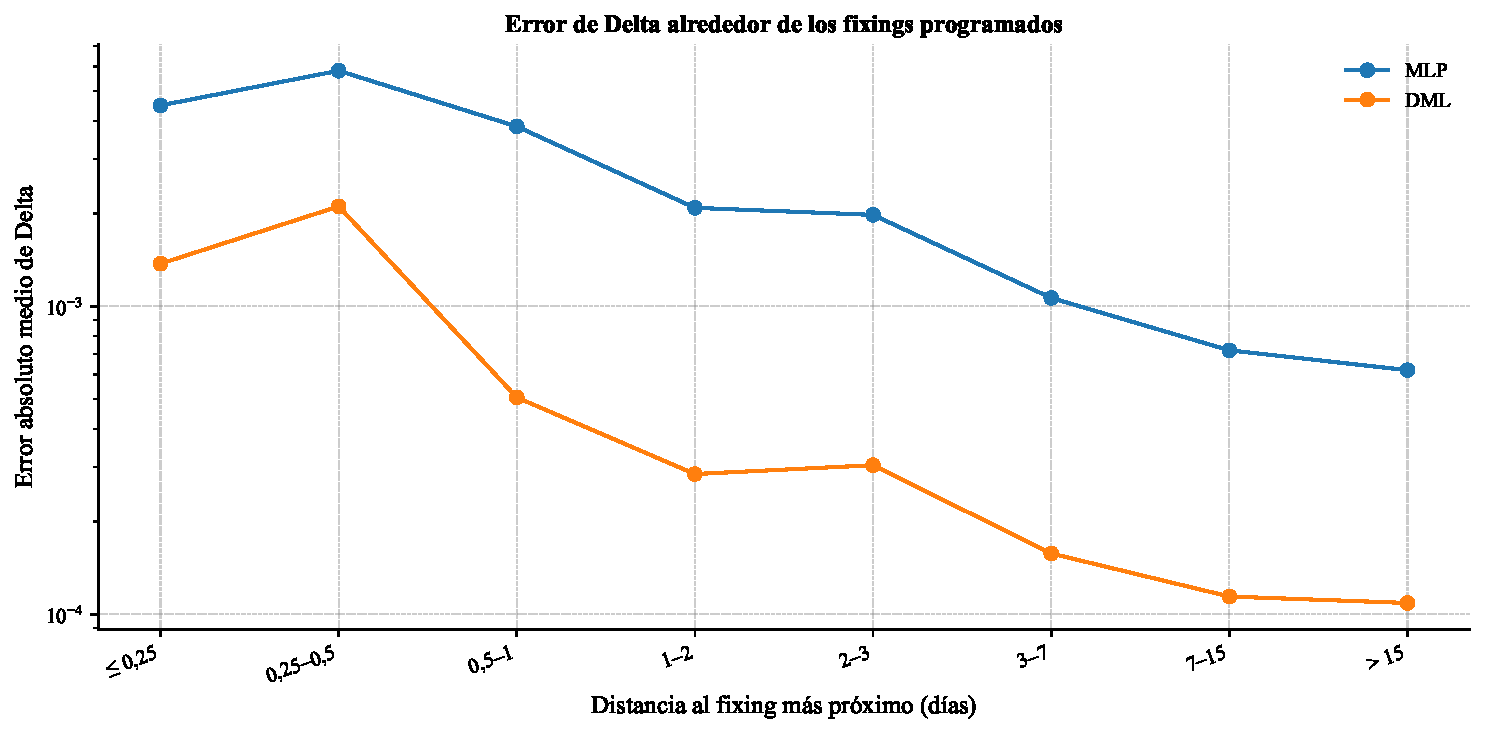
\includegraphics[width=0.86\textwidth]{../figures/ml/04_fixing_boundary_delta_error.pdf}
    \caption{Error absoluto medio de Delta según la distancia a la frontera de fixing más próxima.}
    \label{fig:fixing_boundary_delta_error}
\end{figure}

La correlación de Spearman entre $|\varepsilon^\Delta_{DML}|$ y
$d_{\mathrm{fix}}$ en todo el diagnóstico es sólo $-0{,}161$. Por tanto, la proximidad a
un fixing no explica globalmente el error de Delta; su efecto aparece sobre todo en la cola.
DML mantiene además menor error que MLP en todos los intervalos, por lo que el problema
parece asociado a la representación del régimen contractual más que a una pérdida de la
ventaja relativa de DML.

El patrón se mantiene cualitativamente en referencia, aunque con menor concentración. La
interpretación es que, con el calendario fijo, $\tau$ determina toda la información
temporal de los fixings. Una codificación explícita de $n_{\mathrm{fix}}^{\mathrm{future}}$ y $d_{\mathrm{fix}}$ podría
facilitar la representación de los cambios discretos de régimen sin añadir información. Esta modificación no se
implementa por haber sido identificada después de congelar el protocolo y queda como
extensión futura.

\section{Cobertura local: transmisión económica de la mejora en Delta}
\label{sec:local_hedging}

La cobertura local estudia si la mayor precisión de Delta se traduce en una menor exposición
de primer orden ante perturbaciones pequeñas. Para un shock $\Delta P$ se evalúa
\begin{equation}
    \varepsilon_{\mathrm{hedge}}
    =
    \Delta V-\widehat{\Delta}_t\,\Delta P,
    \label{eq:local_hedge_residual_results}
\end{equation}
frente al residuo sin cobertura $\Delta V$. Se comparan no-hedge, MLP, DML y una Delta
Oracle RQMC. El shock principal es 1\%, con 0{,}5\% y 2\% como robustez.

\begin{table}[htbp]
\centering
\small
\caption{RMSE de cobertura local según magnitud del shock}
\label{tab:local_hedge_rmse}
\begin{tabular}{lcccc}
\toprule
\textbf{Shock}
& \textbf{Sin cobertura}
& \textbf{MLP}
& \textbf{DML}
& \textbf{Oracle RQMC} \\
\midrule
$0{,}5\%$
& $6{,}7744\times10^{-5}$
& $3{,}3379\times10^{-6}$
& $5{,}0278\times10^{-7}$
& $8{,}9543\times10^{-8}$ \\
$1{,}0\%$
& $1{,}3549\times10^{-4}$
& $6{,}6878\times10^{-6}$
& $1{,}0584\times10^{-6}$
& $3{,}4914\times10^{-7}$ \\
$2{,}0\%$
& $2{,}7096\times10^{-4}$
& $1{,}3428\times10^{-5}$
& $2{,}4162\times10^{-6}$
& $1{,}3738\times10^{-6}$ \\
\bottomrule
\end{tabular}
\end{table}

Con el shock del 1\%, DML reduce el RMSE aproximadamente 84{,}2\% frente al
MLP y 99{,}2\% frente a no cubrir. El MAE confirma la misma jerarquía:
$1{,}2003\times10^{-4}$ (no-hedge), $4{,}4943\times10^{-6}$ (MLP),
$8{,}2692\times10^{-7}$ (DML) y $2{,}6240\times10^{-7}$ (Oracle), lo que
supone una mejora de DML del 81{,}6\% respecto al MLP. En 12\,280
comparaciones emparejadas del shock principal, DML supera al MLP en 86{,}1\% y al
no-hedge en 97{,}5\%. La ordenación del RMSE se mantiene para los tres tamaños de shock
y en los cuatro bloques físicos independientes.

El Oracle permanece por debajo de DML, pero la distancia entre MLP y el benchmark
numérico se reduce de forma sustancial. El resultado establece una traducción económica
clara de la mejora de Delta en un problema local de primer orden. Su alcance es
limitado a estados interiores del calendario. La dinámica añade rebalanceo y
acumulación temporal y evalúa en fronteras de fixing. El cambio simultáneo de diseño
y muestra impide atribuir el deterioro a un único componente.

\section{Cobertura dinámica con forwards}
\label{sec:dynamic_hedging}

La prueba dinámica rebalancea mensualmente, después de cada fixing, un forward de compute
modelizado y de coste inicial nulo. Se comparan no-hedge, Oracle RQMC y los ensembles de
cinco semillas MLP y DML entrenados con 65\,536 estados. Tras exigir permanencia en el
dominio común válido, la evaluación comprende 2\,038 trayectorias terminales. El diseño fue
fijado antes de observar los resultados y no se aplicó \textit{clipping}, reentrenamiento ni
sustitución posterior del instrumento.

\begin{table}[htbp]
\centering
\small
\caption{Distribución del error terminal en la cobertura dinámica}
\label{tab:dynamic_forward_distribution}
\resizebox{\textwidth}{!}{%
\begin{tabular}{lccccc}
\toprule
\textbf{Estrategia}
& \textbf{RMSE}
& \textbf{MAE}
& \textbf{Mediana $|E_T|$}
& \textbf{P95 $|E_T|$}
& \textbf{P99 $|E_T|$} \\
\midrule
Sin cobertura
& $0{,}014998$
& $0{,}011973$
& $0{,}011046$
& $0{,}032054$
& $0{,}046658$ \\
Oracle RQMC
& $0{,}002311$
& $0{,}001742$
& $0{,}001356$
& $0{,}004684$
& $0{,}006682$ \\
MLP
& $0{,}106515$
& $0{,}035403$
& $0{,}003345$
& $0{,}208294$
& $0{,}460250$ \\
DML
& $0{,}038698$
& $0{,}013641$
& $0{,}002117$
& $0{,}078235$
& $0{,}194261$ \\
\bottomrule
\end{tabular}
}
\end{table}

El RMSE produce una ordenación distinta de la cobertura local:
\begin{equation}
    RMSE_{\mathrm{Oracle}}
    <
    RMSE_{0}
    <
    RMSE_{\mathrm{DML}}
    <
    RMSE_{\mathrm{MLP}}.
    \label{eq:dynamic_rmse_order}
\end{equation}
El Oracle reduce el RMSE un 84{,}6\% frente a no cubrir, lo que demuestra que el
mecanismo puede reducir riesgo dentro del entorno modelizado. DML reduce el RMSE
63{,}7\% frente al MLP, pero permanece por encima del no-hedge. Sin embargo, la mediana
absoluta de DML es 0{,}002117 frente a 0{,}011046 sin cobertura, y DML obtiene menor
$|E_T|$ que el MLP en 70{,}07\% de las trayectorias y que el no-hedge en 77{,}33\%.
La aparente contradicción entre comportamiento típico y RMSE se debe a la severidad de la
cola: P99 es 0{,}194261 para DML frente a 0{,}046658 sin cobertura y 0{,}460250 para
MLP; los máximos alcanzan 0{,}470193, 0{,}073272 y 1{,}683016, respectivamente.

La ventaja de DML en Delta persiste durante los rebalanceos, como muestra la
Figura~\ref{fig:dynamic_delta_fixings}: su RMSE de sensibilidad permanece por debajo del
MLP en todas las fronteras representadas. Por tanto, el peor RMSE terminal no se explica por
una inversión de la jerarquía MLP--DML en Delta.

\begin{figure}[htbp]
    \centering
    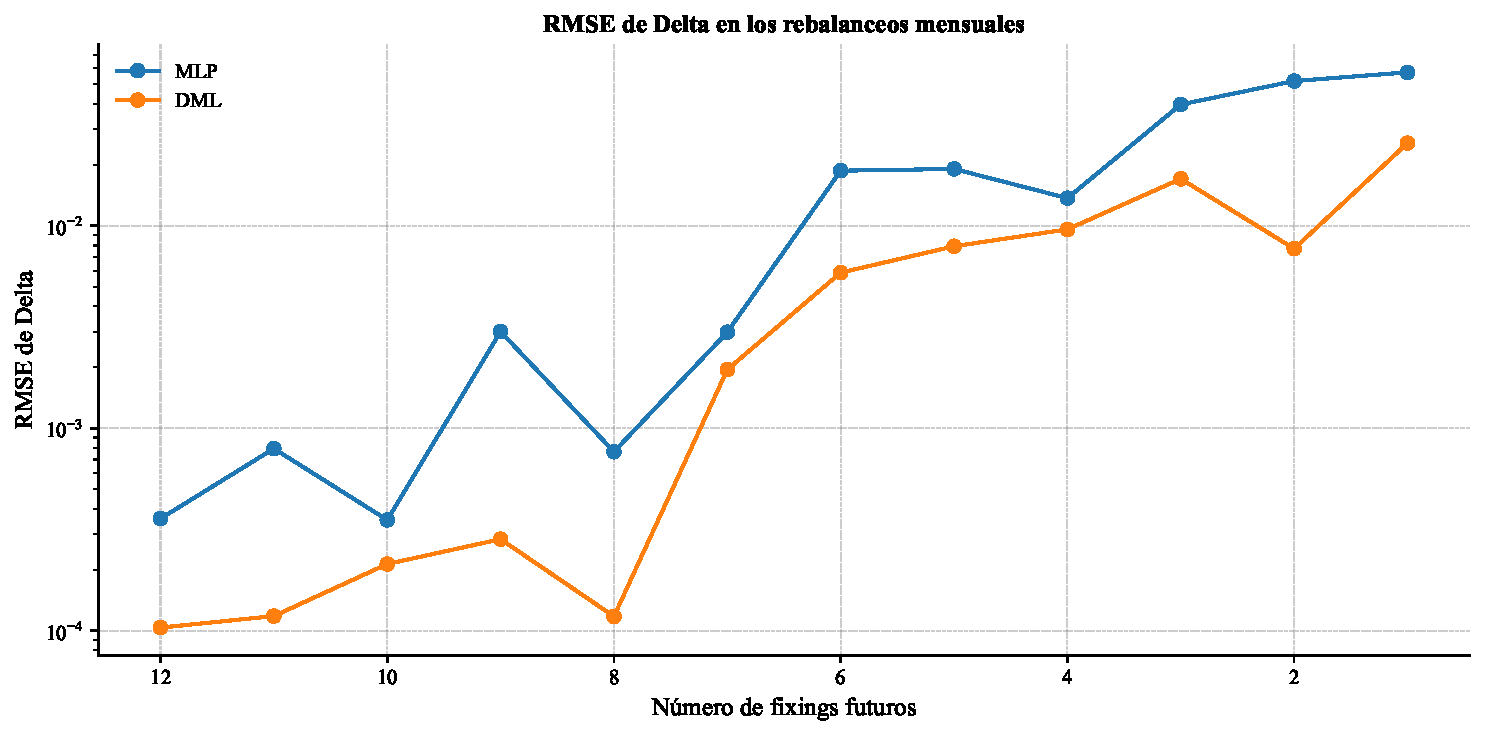
\includegraphics[width=0.80\textwidth]
    {../figures/hedging/08_dynamic_delta_error_by_fixing.pdf}
    \caption{RMSE de Delta frente al benchmark RQMC según el número de
    fixings futuros en la cobertura dinámica.}
    \label{fig:dynamic_delta_fixings}
\end{figure}

La transformación desde Delta a unidades de forward constituye un mecanismo relevante. Si
$J_t^F=\partial F_t/\partial P_t$, la posición histórica ejecutada y su desviación respecto a la misma política de
referencia son
\begin{align}
    \widehat h_t &= \frac{\widehat{\Delta}_t}{J_t^F},
    \label{eq:dynamic_hedge_ratio}\\
    \widehat h_t-h_t^*
    &=\frac{\widehat\Delta_t-\Delta_t^*}{J_t^F}.
    \label{eq:hedge_ratio_error_amplification}
\end{align}
Cuando $|J_t^F|$ es pequeño, errores moderados de Delta pueden amplificarse al
convertirse en unidades del instrumento de cobertura. Este mecanismo es compatible con una
dinámica fuertemente mean-reverting, pero no identifica causalmente cada trayectoria extrema.
El diseño combina rebalanceo discreto, transiciones de fixing y acumulación temporal,
sin estimar sus contribuciones causales por separado. El forward se liquida sobre el
mismo índice simulado de la asiática: no se introduce un factor de base independiente.

La comparación con el Oracle es esencial: utilizando el mismo calendario y forward, su RMSE
de 0{,}002311 es muy inferior al no-hedge. Por tanto, el resultado de MLP y DML no implica
que la cobertura con el forward sea incapaz de funcionar por construcción. A la vez, el forward
es un instrumento \emph{modelizado}; el experimento no demuestra liquidez ni disponibilidad
de un contrato real equivalente.

La corrección del descuento de la Ecuación~\ref{eq:forward_pv_correction}
se evalúa como diagnóstico posterior sobre las mismas liquidaciones conservadas.
Con $r=0{,}03$ y $h=1/12$, multiplica cada posición por
$e^{rh}=1{,}00250313$. Los RMSE resultantes son $0{,}002309264$ para Oracle,
$0{,}106781890$ para MLP y $0{,}038794595$ para DML, frente a los valores
históricos $0{,}002310699$, $0{,}106515000$ y $0{,}038698442$.
La jerarquía permanece y la omisión no explica las colas. Esta reponderación
algebraica conserva estados, Deltas y prima inicial; no sustituye al protocolo original.

En las 24\,456 decisiones dinámicas de cada estrategia aparecen 90 Deltas
negativas del ensemble DML, 1187 del MLP y ninguna del Oracle. Este diagnóstico
no identifica qué parte de la cola causan dichas violaciones.

\section{Concentración del error en las colas}
\label{sec:tail_concentration}

Para cuantificar cuánto pesa una fracción pequeña de trayectorias en el RMSE se define
\begin{equation}
    C_q^{(s)}
    =
    \frac{\sum_{i\in\mathcal{T}_{q,s}}E_{i,s}^{2}}
         {\sum_{i=1}^{N}E_{i,s}^{2}},
    \label{eq:mse_concentration}
\end{equation}
donde $\mathcal{T}_{q,s}$ contiene el porcentaje $q$ de trayectorias con mayor
$|E_{i,s}|$. En las 2\,038 trayectorias finales, el peor 1\% representa 21
realizaciones y el peor 5\% unas 102.

\begin{figure}[htbp]
    \centering
    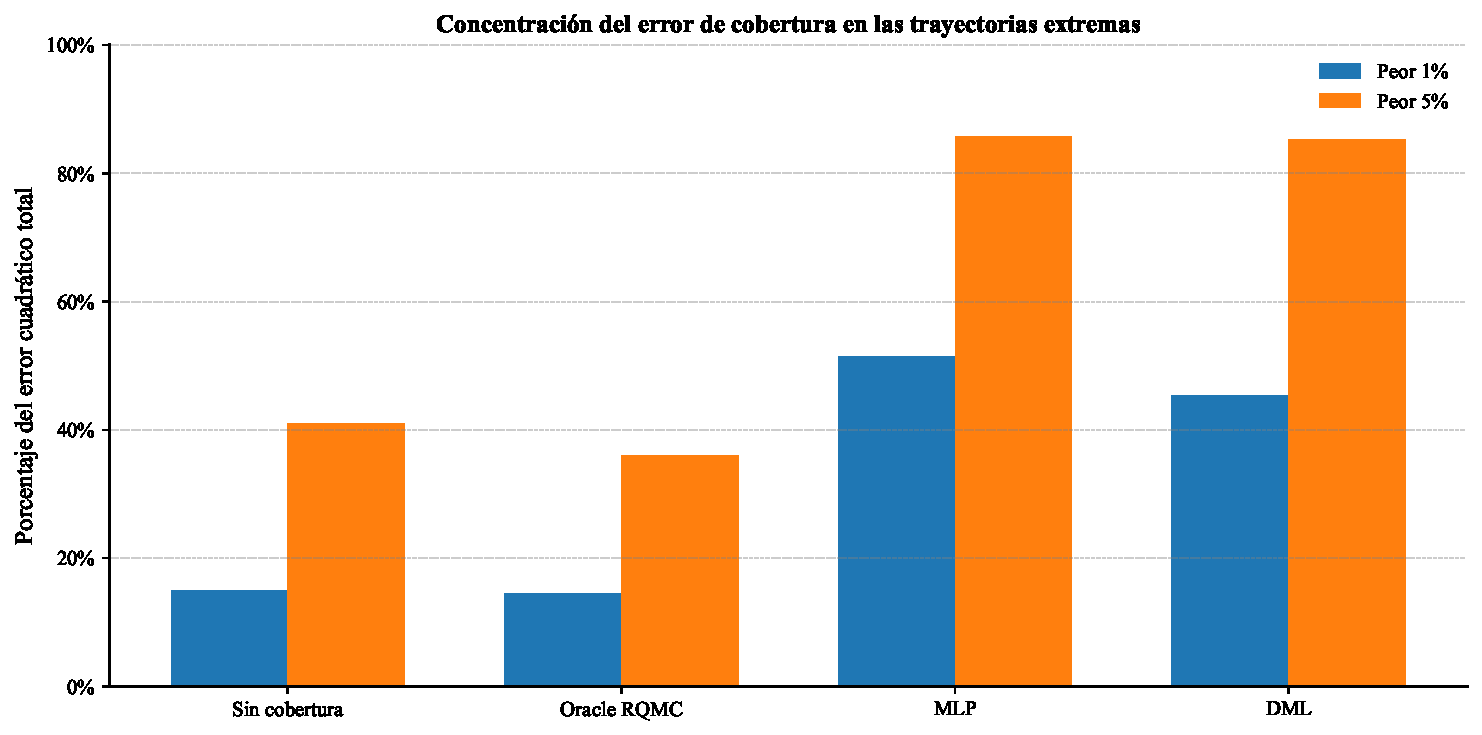
\includegraphics[width=0.80\textwidth]
    {../figures/hedging/07_dynamic_tail_concentration.pdf}
    \caption{Concentración del error cuadrático terminal en las trayectorias
    extremas.}
    \label{fig:dynamic_tail_concentration}
\end{figure}

En DML, aproximadamente 45--46\% del error cuadrático total procede del peor
1\% y alrededor del 85\% del peor 5\%. Para MLP las proporciones son
aproximadamente 51--52\% y 86\%; para no-hedge, 15\% y 41\%; y para
Oracle, 15\% y 36\%. Así, unas 102 trayectorias explican alrededor del
85\% de la suma de errores cuadrados de DML.

Este diagnóstico reconcilia las métricas dinámicas: DML mejora al no-hedge en 77{,}33\%
de las trayectorias y reduce sustancialmente la mediana, pero una fracción muy pequeña de
realizaciones adversas domina el RMSE. DML reduce además la severidad de la cola frente al
MLP, aunque no la elimina. La evidencia es compatible con la interacción entre error residual
de Delta, posible amplificación por $(J_t^F)^{-1}$, fronteras de fixing y acumulación temporal;
no permite atribuir causalmente la cola a uno solo de estos mecanismos.

\section{Discusión conjunta y robustez}
\label{sec:joint_discussion}

La Tabla~\ref{tab:joint_results_summary} resume la evidencia que responde a las preguntas
del trabajo. El patrón no es de dominancia uniforme, sino de una ventaja diferencial que es
débil en pricing, fuerte en Delta y cobertura local, y condicionada por las colas en cobertura
dinámica.

\begin{table}[htbp]
\centering
\small
\caption{Síntesis de los principales resultados de la configuración final}
\label{tab:joint_results_summary}
\begin{tabular}{>{\raggedright\arraybackslash}p{2.6cm}>{\raggedright\arraybackslash}p{2.8cm}>{\raggedright\arraybackslash}p{2.8cm}>{\raggedright\arraybackslash}p{4.6cm}}
\toprule
\textbf{Dimensión}
& \textbf{MLP}
& \textbf{DML}
& \textbf{Interpretación} \\
\midrule
Precio, test
&
RMSE $=0{,}001624$

MAE $=0{,}000123$
&
RMSE $=0{,}001516$

MAE $=0{,}000136$
&
DML mejora RMSE, pero MLP obtiene menor MAE: no existe dominancia uniforme. \\[1.5mm]
Delta, test
&
RMSE $=0{,}008528$

MAE $=0{,}001234$
&
RMSE $=0{,}001817$

MAE $=0{,}000216$
&
Ventaja amplia y sistemática de DML en la sensibilidad. \\[1.5mm]
Cobertura local, shock $1\%$
&
RMSE $=6{,}69\times10^{-6}$
&
RMSE $=1{,}06\times10^{-6}$
&
La mejora de Delta se transmite claramente a la neutralización local. \\[1.5mm]
Cobertura dinámica
&
RMSE $=0{,}106515$
&
RMSE $=0{,}038698$
&
DML mejora fuertemente al MLP, pero no supera al no-hedge
($RMSE=0{,}014998$) por la severidad de una cola reducida. \\
\bottomrule
\end{tabular}
\end{table}

La robustez interna procede de varias dimensiones complementarias. En Delta, DML gana las
cinco semillas para los cuatro tamaños de entrenamiento y la conclusión se reproduce con
etiquetas de referencia de mayor precisión. En cobertura local, la jerarquía
Oracle--DML--MLP--no-hedge se mantiene para shocks de 0{,}5\%, 1\% y 2\% y
en los cuatro bloques físicos. Los diagnósticos de fixing y concentración de cola se realizaron
sobre modelos congelados y no se utilizaron para modificar el protocolo.

Las conclusiones fuertes son, por tanto, que DML mejora de forma amplia y robusta la Delta
y que esa mejora tiene una traducción económica clara en cobertura local. En pricing, la
evidencia es mixta; en cobertura dinámica, DML mejora sustancialmente al MLP y el
comportamiento típico, pero no domina al no-hedge en RMSE. De aquí se desprende el
resultado conceptual principal:
\[
    \text{una Delta más precisa no implica automáticamente un hedge dinámico superior.}
\]
La eficacia final depende también del instrumento utilizado, del calendario contractual y de la
acumulación de errores.

